\section{Постановка задачі автоматизації на основі єдиного методологічного підходу}

\subsubsection{Гіроскопічний датчик кута}

Гіроскопічний датчик кута \nomenclature{ДК}{датчик кута}, 
за допомогою якого задається направлення об’єкту 
стабілізації $\varphi_\text{з}$ і вимірюється розузгодження 
$\Theta_0 = \varphi_\text{з} - \varphi_0$ , при роботі в режимі стабілізації 
є практично безінерційною ланкою (рис. \ref{fig:angle sensor}). Його передаточна 
функція має вигляд:

$$ W_\text{ДК} = \frac{U_\text{у}}{\Theta_0} = \frac{U_\text{у}}{\varphi_\text{з} - \varphi_0} = k_\text{ВТК} $$

\begin{figure}
\centering
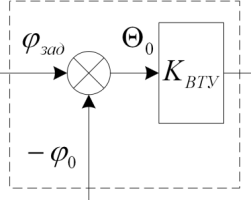
\includegraphics[scale=0.5]{angle_sensor}
\caption{Структурна схема датчика кута}
\label{fig:angle sensor}
\end{figure} 

